\documentclass{article}
\usepackage{amsmath}
\usepackage{graphicx} % Required for inserting images
\usepackage{enumerate}
\usepackage{ctex}
\usepackage{romannum}
\usepackage[colorlinks=true, allcolors=magenta]{hyperref}
\usepackage[legalpaper, margin=100pt]{geometry}
\usepackage{setspace}
\usepackage{tcolorbox}
\renewcommand{\baselinestretch}{1.25}

\setlength{\parindent}{20pt}

\title{第二幕~度量}
\author{Wayne Zheng}
\date{\today}

\begin{document}

\maketitle
\tableofcontents

\section{曲面映射:度量}

\emph{度量}(Metric):也被称为\emph{第一基本形式}(first fundamental form),表示两个临近点之间的无穷小距离的参数化规则。
参数化的规则选取可以有很多种,因此每个曲面原则上可以写下无穷多种度量。
度量决定了曲面的内蕴几何,这是高斯最早对微分几何的基本见解。

例如,平面可以有无穷多种度量,直角坐标系中$d\hat{s}^{2}=dx^{2}+dy^{2}$,极坐标中是$d\hat{s}^{2}=dr^{2}+r^{2}d\theta^{2}$.
其对应的\emph{度量张量}(metric tensor)分别为:
\begin{equation}
g=
\begin{pmatrix}
1 & 0 \\
0 & 1
\end{pmatrix}, \quad
g=
\begin{pmatrix}
1 & 0 \\
0 & r^{2}
\end{pmatrix}.
\end{equation}

下面我们看球面的例子。
我们先考虑球坐标系$(\phi, \theta)$,其中$\phi\in[0, \pi]$是极角,表示纬度的取值范围;$\theta\in[0, 2\pi)$是方位角,表示经度的取值范围。
我们先来看几何直观。

\begin{figure}[htbp]
    \centering % 图片居中
    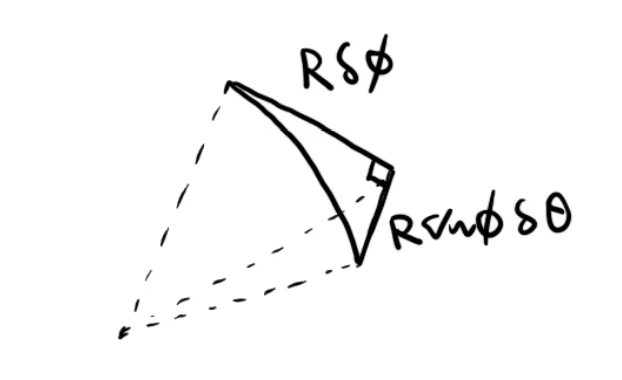
\includegraphics[width=0.3\textwidth]{../figs/chap4_01.jpg} % 图片路径
    \caption{球坐标系下的度量。} 
    \label{fig:chap4_01} 
\end{figure}

由图~\ref{fig:chap4_01}可知,球面上无穷小两点之间的距离可以表示为$d\hat{s}^{2}=\left(Rd\phi\right)^{2}+\left(R\sin\phi{d}\theta\right)^{2}$.


然后,让我们严格地详细计算这个度量。
球面上的一点$(x, y, z)$可以用球坐标参数化,即
\begin{equation*}
(x(\phi, \theta), y(\phi, \theta), z(\phi, \theta))=(R\sin\phi\cos\theta, R\sin\phi\sin\theta, R\cos\phi).
\end{equation*}
进一步地,球面上任意一条曲线可以用一个参数参数化,即$\mathbf{r}=\mathbf{r}(t)=\mathbf{r}(\phi(t), \theta(t))$.
其切向量为:$\mathbf{r}^{\prime}(t)=\partial_{\phi}\mathbf{r}\dot{\phi}+\partial_{\theta}\mathbf{r}\dot{\theta}$.
其中两个极坐标参数的切向量为:
\begin{equation}
\begin{aligned}
\mathbf{r}_{\phi}
&=\frac{\partial\mathbf{r}}{\partial\phi}
=\left(R\cos\phi\cos\theta, R\cos\phi\sin\theta, -R\sin\phi\right), \\
\mathbf{r}_{\theta}
&=\frac{\partial\mathbf{r}}{\partial\theta}
=\left(-R\sin\phi\sin\theta, R\sin\phi\cos\theta, 0\right).
\end{aligned}
\end{equation}
球面度量为
\begin{equation*}
\begin{aligned}
d\hat{s}^{2}
&=dx^{2}+dy^{2}+dz^{2} \\
&=\left(\partial_{\phi}{x}d\phi+\partial_{\theta}{x}d\theta\right)^{2}+\left(\partial_{\phi}{y}d\phi+\partial_{\theta}{y}d\theta\right)^{2}+\left(\partial_{\phi}{z}d\phi+\partial_{\theta}{z}d\theta\right)^{2} \\
&=\mathbf{r}_{\phi}\cdot\mathbf{r}_{\phi}d\phi^{2}+\mathbf{r}_{\theta}\cdot\mathbf{r}_{\theta}d\theta^{2}+\mathbf{r}_{\phi}\cdot\mathbf{r}_{\theta}d\phi{d}\theta+\mathbf{r}_{\theta}\cdot\mathbf{r}_{\phi}d\theta{d}\phi.
\end{aligned}
\end{equation*}
则其度量张量为
\begin{equation}
g=\begin{pmatrix}
g_{\phi\phi} & g_{\phi\theta} \\
g_{\theta\phi} & g_{\theta\theta}
\end{pmatrix}
=\begin{pmatrix}
\mathbf{r}_{\phi}\cdot\mathbf{r}_{\phi} & \mathbf{r}_{\phi}\cdot\mathbf{r}_{\theta} \\
\mathbf{r}_{\theta}\cdot\mathbf{r}_{\phi} & \mathbf{r}_{\theta}\cdot\mathbf{r}_{\theta}
\end{pmatrix}
=\begin{pmatrix}
R^{2} & 0 \\
0 & R^{2}\sin^{2}\phi
\end{pmatrix}.
\end{equation}
最终,球面用$(\phi, \theta)$写下的度量为$d\hat{s}^{2}=R^{2}\left(d\phi^{2}+\sin^{2}\phi{d}\theta^{2}\right)$,与几何直观方法得到的一致。

类似地,我们计算中心投影的度量(习题3)。首先是用切平面上的参数$(r, \theta)$来参数化球面上的点:
\begin{equation*}
\begin{aligned}
\mathbf{l}=(x, y, z)
&=(R\sin\phi\cos\theta, R\sin\phi\sin\theta, R\cos\phi) \\
&=\left(\frac{Rr\cos\theta}{\sqrt{R^{2}+r^{2}}}, \frac{Rr\sin\theta}{\sqrt{R^{2}+r^{2}}}, \frac{R^{2}}{\sqrt{R^{2}+r^{2}}}\right).
\end{aligned}
\end{equation*}
相应地,可以计算切向量$\mathbf{l}_{r}=\partial_{r}\mathbf{l}, \mathbf{l}_\theta=\partial_{\theta}\mathbf{l}$.
度量张量为
\begin{equation}
g=\begin{pmatrix}
g_{r\phi} & g_{r\theta} \\
g_{\theta{r}} & g_{\theta\theta}
\end{pmatrix}
=\begin{pmatrix}
\mathbf{l}_{r}\cdot\mathbf{l}_{r} & \mathbf{l}_{r}\cdot\mathbf{l}_{\theta} \\
\mathbf{l}_{\theta}\cdot\mathbf{l}_{r} & \mathbf{l}_{\theta}\cdot\mathbf{l}_{\theta}
\end{pmatrix}
=\begin{pmatrix}
\frac{R^{4}}{\left(R^{2} + r^{2}\right)^{2}} & 0 \\
0 & \frac{R^{2}r^{2}}{R^{2} + r^{2}}
\end{pmatrix}.
\end{equation}
则其度量为
\begin{equation}
d\hat{s}^{2}=\frac{R^{4}}{\left(R^{2}+r^{2}\right)^{2}}dr^{2}+\frac{R^{2}r^{2}}{R^{2}+r^{2}}d\theta^{2}
=\frac{1}{1+(r/R)^{2}}\left[\frac{dr^{2}}{1+(r/R)^{2}}+r^{2}d\theta^{2}\right],
\end{equation}
与几何直观方法得到的一致。

\begin{figure}[htbp]
    \centering % 图片居中
    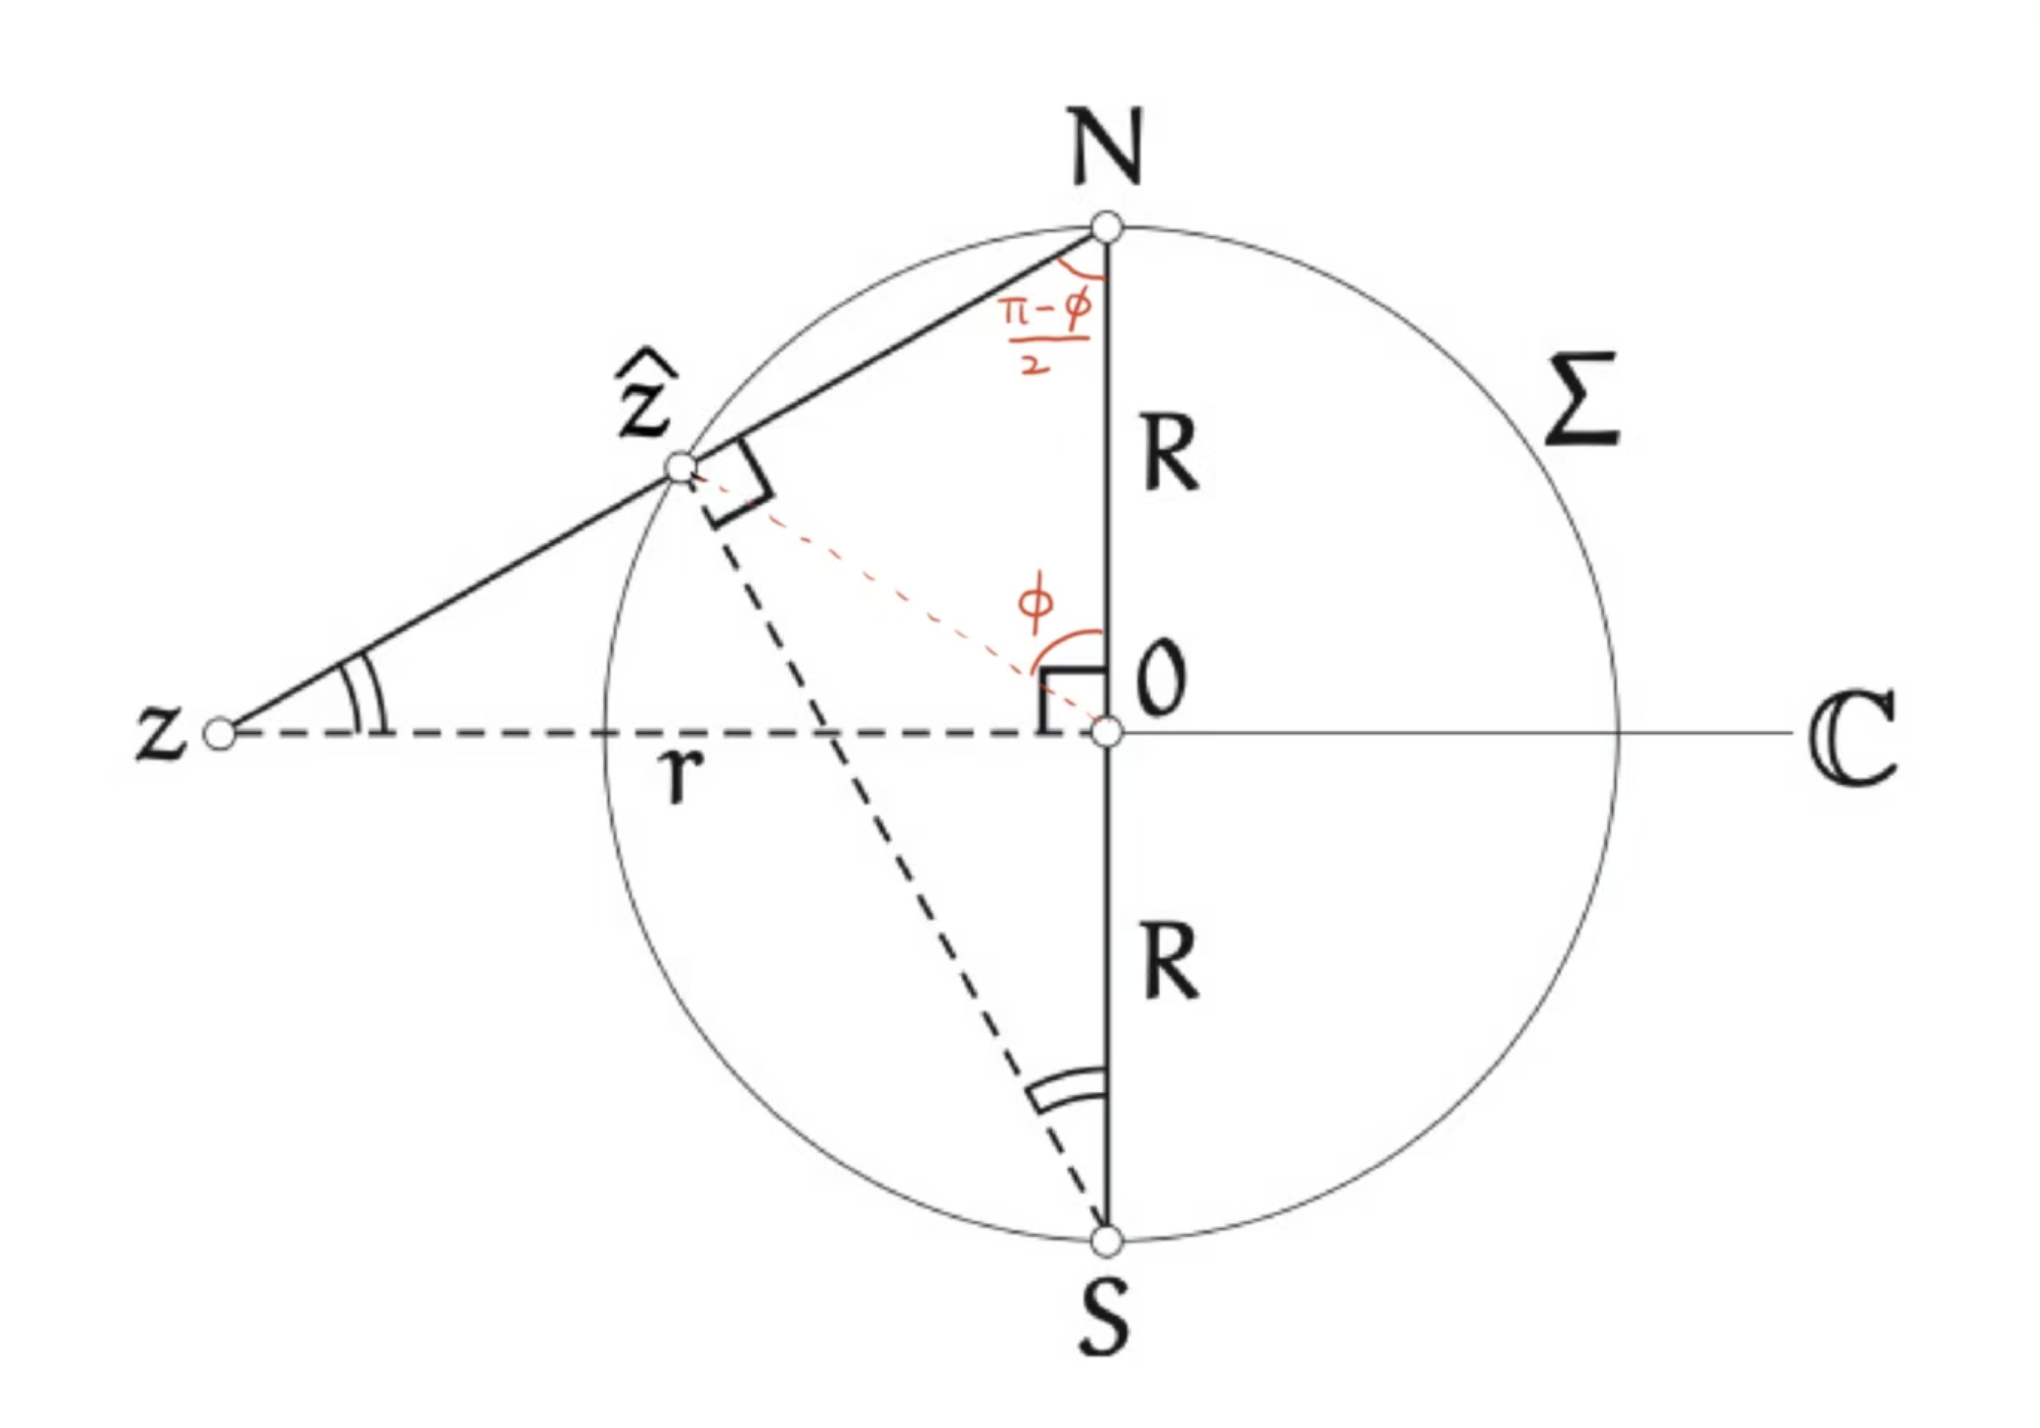
\includegraphics[width=0.5\textwidth]{../figs/chap4_02.png}
    \caption{球极投影的侧剖图。} 
    \label{fig:chap4_02} 
\end{figure}

我们再来计算球极投影的度量。
如图~\ref{fig:chap4_02}所示,我们有:
\begin{equation*}
\sin\left(\frac{\pi-\phi}{2}\right)
=\cos\left(\frac{\phi}{2}\right)=\frac{r}{\sqrt{R^{2}+r^{2}}}, \quad
\cos\left(\frac{\pi-\phi}{2}\right)
=\sin\left(\frac{\phi}{2}\right)=\frac{R}{\sqrt{R^{2}+r^{2}}}.
\end{equation*}
球极投影的参数化为
\begin{equation*}
\begin{aligned}
\mathbf{l}=(x, y, z)
&=(R\sin\phi\cos\theta, R\sin\phi\sin\theta, R\cos\phi) \\
&=\left[\frac{2R^{2}r\cos\theta}{R^{2}+r^{2}}, \frac{2R^{2}r\sin\theta}{R^{2}+r^{2}}, \frac{R(r^{2}-R^{2})}{R^{2}+r^{2}}\right].
\end{aligned}
\end{equation*}
相应地,可以计算切向量$\mathbf{l}_{r}=\partial_{r}\mathbf{l}, \mathbf{l}_\theta=\partial_{\theta}\mathbf{l}$.
度量张量为
\begin{equation}
g=\begin{pmatrix}
g_{r\phi} & g_{r\theta} \\
g_{\theta{r}} & g_{\theta\theta}
\end{pmatrix}
=\begin{pmatrix}
\mathbf{l}_{r}\cdot\mathbf{l}_{r} & \mathbf{l}_{r}\cdot\mathbf{l}_{\theta} \\
\mathbf{l}_{\theta}\cdot\mathbf{l}_{r} & \mathbf{l}_{\theta}\cdot\mathbf{l}_{\theta}
\end{pmatrix}
=\begin{bmatrix}
\frac{4R^{4}}{\left(R^{2} + r^{2}\right)^{2}} & 0 \\
0 & \frac{4R^{4}r^{2}}{\left(R^{2} + r^{2}\right)^{2}}
\end{bmatrix}.
\end{equation}
则其度量为$d\hat{s}^{2}=\frac{4R^{4}}{\left(R^{2} + r^{2}\right)^{2}}\left(dr^{2}+r^{2}d\theta^{2}\right)$.
即$d\hat{s}=\frac{2R^{2}}{R^{2} + r^{2}}ds$,是一个共形变换,与几何直观方法得到的一致。

\begin{tcolorbox}[colback=white, arc=3mm, auto outer arc]
\begin{minipage}[c,t]{1.0\textwidth}
\kaishu
设平面的方程为:
\begin{equation*}
    Ax+By+Cz=D.
\end{equation*}
设$P=(x_{0}, y_{0}, z_{0})$ 与$Q=(x_{1}, y_{1}, z_{1})$是平面上的两点,$\mathbf{v}\equiv(x_{1}-x_{0}, y_{1}-y_{0}, z_{1}-z_{0})$.
则显然$\mathbf{v}$与$\mathbf{n}=(A, B, C)$正交,即$\mathbf{v}\cdot\mathbf{n}=0$.
$\mathbf{n}$是平面的法向量。
另设$P^{\prime}=(x_{0}^{\prime}, y_{0}^{\prime}, z_{0}^{\prime})$是平面外的任意一点,则$P^{\prime}$到平面的距离的向量即为投影到法向量方向:$    \mathbf{d}=\text{Proj}_{\mathbf{n}}\left(\overrightarrow{P^{\prime}P}\right)=\vert\overrightarrow{P^{\prime}P}\vert\cos\alpha\hat{\mathbf{n}}$.
距离为
\begin{equation*}
d=\overrightarrow{P^{\prime}P}\cdot\hat{\mathbf{n}}
=\frac{\vert Ax_{0}^{\prime}+By_{0}^{\prime}+Cz_{0}^{\prime}-D\vert}{\sqrt{A^{2}+B^{2}+C^{2}}}.
\end{equation*}
\end{minipage}
\end{tcolorbox}

\section{伪球面和双曲平面}

贝尔特拉米(Beltrami)是意大利数学家,对双曲几何有重要贡献。
他也发现了拉格朗日力学中的贝尔特拉米等式。
他也知道局部的高斯-博内定理。

\subsection{利用变分原理证明广义斯涅尔定律}

\begin{tcolorbox}[colback=white, arc=3mm, auto outer arc]
\begin{minipage}[c,t]{1.0\textwidth}
\kaishu
贝尔特拉米等式。
考虑作用量
\begin{equation*}
    S=\int{L}(u, u^{\prime}, x)dx
\end{equation*}
使函数$u(x)$取到极值。
这里$x$是描述系统演化的独立参数(类比于时间$t$),$u$可以看作是广义坐标。
可以定义广义动量$p=\partial{L}/\partial{u^{\prime}}$.
此时变分原理导出的拉格朗日方程简化为
\begin{equation*}
    \frac{dp}{dx}-\frac{\partial{L}}{\partial{u}}=0.
\end{equation*}
哈密顿量$H=u^{\prime}p-L$.
利用拉格朗日方程,则可以得到贝尔特拉米等式:
\begin{equation*}
\begin{aligned}
\frac{dH}{dx}
&=\left(pu^{\prime\prime}+\frac{dp}{dx}u^{\prime}\right)-\left(\frac{\partial{L}}{\partial{u}}u^{\prime}+\frac{\partial{L}}{\partial{u\prime}}u^{\prime\prime}+\frac{\partial{L}}{\partial{x}}\right)=-\frac{\partial{L}}{\partial{x}}.
\end{aligned}
\end{equation*}
这是诺特定理的一个特例。
\end{minipage}
\end{tcolorbox}

考虑光在介质中的传播,坐标是$(x, y)$,路径可以表示成曲线 $y=y(x)$.
不妨进一步假设折射率只是纵坐标的函数$n=n(y)$.
则光从$A$到$B$的作用量是累积用时的积分
\begin{equation}
\begin{aligned}
S
&=\int\frac{ds}{v}
=\int\frac{1}{v(y)}\sqrt{dx^{2}+dy^{2}} \\
&=\int_{x_{A}}^{x_{B}}n(y)\sqrt{1+\left(\frac{dy}{dx}\right)^{2}}dx
\equiv\int_{x_{A}}^{x_{B}}Ldx,
\end{aligned}
\end{equation}
其中拉氏量$L=n(y)\sqrt{1+y^{\prime{2}}}$.
根据费马变分原理,光线沿着作用量$S$取极值(最小值)的路径。
哈密顿量
\begin{equation}
    H
    =y^{\prime}p-L
    =-\frac{n(y)}{\sqrt{1+y^{\prime{2}}}}.
\end{equation}
根据贝尔特拉米等式,易得$dH/dx=0$,即$H=-k$是一个常数,也就意味着系统沿着$x$方向具有连续的平移不变性,从而对应有一个守恒量,这个守恒量
\begin{equation}
    \frac{n(y)}{\sqrt{1+y^{\prime{2}}}}
    =n(y)\frac{dx}{\sqrt{dx^{2}+dy^{2}}}
    =n(y)\sin\theta=k
\end{equation}
给出了连续介质的斯涅尔定律,$\theta$是光线与入射平面的法线的夹角。
这与几何方法得到的斯涅尔定律一致。

\subsection{广义斯涅尔定律的应用}

下面讨论两个例子。

在贝尔特拉米-庞加莱半平面$(x, y)$中,$y>0$,光速$v(y)=y$,
根据广义斯涅尔定律
\begin{equation*}
    \frac{\sin\theta}{y}
    =\frac{1}{y\sqrt{1+y^{\prime{2}}}}=k.
\end{equation*}
原则上需要求解这个关于$y$的常微分方程:$y^{2}(1+y^{\prime{2}})-1/k^{2}=0$,但实际上我们知道$x^{2}+y^{2}=1/k^{2}\equiv{r^{2}}$.
也容易验证$y=\sqrt{r^{2}-x^{2}}$满足此微分方程。

(习题15)如果光在平面$(x, y)$中传播,光速$v(y)=1/\sqrt{1-y}$,则根据广义斯涅尔定律,
\begin{equation*}
    \frac{\sin\theta}{v(y)}
    =\frac{\sqrt{1-y}}{\sqrt{1+y^{\prime{2}}}}=k.
\end{equation*}
求解这个关于$y$的常微分方程:$k^{2}y^{\prime{2}}+y+k^{2}-1=0$,得到的一般解是
\begin{equation*}
    y(x)
    =-\frac{1}{4k^{2}}\left(x-kC\right)^{2}-k^{2}+1,
\end{equation*}
其中$C$是任意常数。
这是一条开口向下的抛物线,顶点在$\left(kC, 1-k^{2}\right)$处。

\section{等距映射和复数}

等距映射(isometric map)是曲面上保持第一基本形式不变的映射。
包括正向(direct)等距映射和反向(opposite)等距映射。
给定一个曲面$\mathcal{S}$,上面的所有等距变换构成一个群,记作$\mathcal{G}$.
所有正向等距变换构成一个子群,记作$\mathcal{G}_{+}(\mathcal{S})$.
在欧几里德几何中,其正向等距变换是
\begin{equation*}
    E(z)=e^{\text{i}\theta}z+k.
\end{equation*}

莫比乌斯变换(Möbius transformation): $z\mapsto M(z)=\frac{az+b}{cz+d}$.
其中最重要的\emph{复反演}$z\mapsto 1/z$可以被看作是几何反演与复共轭的结合,\emph{几何上是黎曼球面绕实轴旋转$\pi$}.

(习题24)考虑$z^{m}$的伸缩扭转从而证明:$(z^{m})^{\prime}=mz^{m-1}$.

令$z=re^{\mathrm{i}\theta}$, 则$\tilde{z}\equiv f(z)=z^{m}=r^{m}e^{\mathrm{i}m\theta}$.
根据定义,$\delta\tilde{z}\equiv f^{\prime}(z)\delta{z}\equiv ae^{\mathrm{i}\tau}\delta{z}$, 其中$a$是伸缩缝因子,$\tau$是扭转角。

我们首先考虑沿着$r$方向的小变化$\delta{z}=\delta{r}e^{\mathrm{i}\theta}$,则$\tilde{z}\rightarrow(r+\delta{r})^{m}e^{m\mathrm{i}\theta}$.
$(r+\delta{r})^{m}\simeq r^{m}+mr^{m-1}\delta{r}$,从而
\begin{equation*}
\delta\tilde{z}=mr^{m-1}\delta{r}e^{\mathrm{i}m\theta}=mr^{m-1}e^{\mathrm{i}(m-1)\theta}\left(\delta{r}e^{\mathrm{i}\theta}\right),
\end{equation*}
从而可以得到伸缩和扭转因子分别为$a=mr^{m-1},\tau=(m-1)\theta$.
所以$f^{\prime}(z)=ae^{\mathrm{i}\tau}=mr^{m-1}e^{\mathrm{i}(m-1)\theta}=mz^{m-1}$.

再让我们考虑沿着弧线方向的小变化,此时原弧长是$\delta{l}=r\delta\theta$,
$\delta{z}=\delta{l}e^{\mathrm{i}(\theta+\pi/2)}$.
像弧长变化为$r^{m}(m\delta)=mr^{m-1}(r\delta\theta)=mr^{m-1}\delta{l}$, 因此
\begin{equation*}
\delta\tilde{z}=mr^{m-1}\delta{l}e^{\mathrm{i}(m\theta+\pi/2)}=mr^{m-1}e^{\mathrm{i}(m-1)\theta}\left[\delta{l}e^{\mathrm{i}(\theta+\pi/2)}\right].
\end{equation*}
从而可以得到伸缩和扭转因子分别为$a=mr^{m-1},\tau=(m-1)\theta$, 与前一致。
这也再次说明$f^{\prime}(z)$不依赖于$\delta{z}$的角度,是\emph{解析共形的}。

%\bibliographystyle{unsrt}
%\bibliography{refs}
\end{document}